\documentclass[a4paper,fleqn,12pt]{article}
%\usepackage[T1]{fontenc}
\usepackage[brazilian]{babel}
%\usepackage[utf8]{inputenc}
\usepackage[left=2.5cm,right=2.5cm,top=3cm,bottom=2.5cm]{geometry}
\usepackage{mathtools}
%\usepackage{amsthm}
%\usepackage{amsmath}
%\usepackage{nccmath}
%\usepackage{amssymb}
\usepackage{amsfonts}
\usepackage{physics}
%\usepackage{dsfont}
%\usepackage{mathrsfs}

\usepackage{titling}
\usepackage{indentfirst}

\usepackage{bm}
\usepackage[dvipsnames]{xcolor}
\usepackage{cancel}

\usepackage{xurl}
\usepackage[colorlinks=true]{hyperref}

% code
\definecolor{bg}{rgb}{0.90,0.90,0.90}
\usepackage{minted}


%\usepackage{float}
%\usepackage{graphicx}
%\usepackage{tikz}
%\usepackage{caption}
%\usepackage{subcaption}

%%%%%%%%%%%%%%%%%%%%%%%%%%%%%%%%%%%%%%%%%%%%%%%%%%%

\newcommand{\eps}{\epsilon}
\newcommand{\vphi}{\varphi}
\newcommand{\cte}{\text{cte}}

\newcommand{\N}{\mathbb{N}}
\newcommand{\Z}{\mathbb{Z}}
\newcommand{\Q}{\mathbb{Q}}
\newcommand{\R}{\mathbb{R}}
%\newcommand{\C}{\mathbb{C}}
\renewcommand{\H}{\hat{H}}
\newcommand{\intR}{\int_{-\infty}^{\infty}}

\newcommand{\0}{\vb{0}}
\newcommand{\1}{\mathds{1}}
\newcommand{\E}{\vb{E}}
\newcommand{\B}{\vb{B}}
\renewcommand{\v}{\vb{v}}
\renewcommand{\r}{\vb{r}}
\renewcommand{\k}{\vb{k}}
\newcommand{\p}{\vb{p}}
\newcommand{\q}{\vb{q}}
\newcommand{\F}{\vb{F}}

\renewcommand{\a}{\hat{a}}
\renewcommand{\b}{\hat{b}}
\renewcommand{\c}{\hat{c}}
\newcommand{\nn}{\hat{n}}

\newcommand{\gf}[2]{\ev{\ev{#1 : #2}}}
\newcommand{\zub}[2]{\ev{\comm{#1}{#2}_\mp}}

\newcommand{\s}[1]{\mathcal{#1}}
%\newcommand{\prodint}[2]{\left\langle #1 , #2 \right\rangle}
\newcommand{\cc}[1]{\overline{#1}}
\newcommand{\Eval}[3]{\eval{\left( #1 \right)}_{#2}^{#3}}

\newcommand{\unit}[1]{\; \mathrm{#1}}

\newcommand{\n}{\medskip}
\newcommand{\e}{\quad \mathrm{e} \quad}
\newcommand{\ou}{\quad \mathrm{ou} \quad}
\newcommand{\virg}{\, , \;}
\newcommand{\ptodo}{\forall \,}
\renewcommand{\implies}{\; \Rightarrow \;}
%\newcommand{\eqname}[1]{\tag*{#1}} % Tag equation with name

% math %
\renewcommand{\erf}[1]{\text{erf}\left(#1\right)}
\newcommand{\floor}[1]{\left\lfloor #1 \right\rfloor}
\newcommand{\ceil}[1]{\left\lceil #1 \right\rceil}

\setlength{\droptitle}{-6em}


\title{\Huge{\textbf{P2 - Statistical Learning}}}
\author{Mateus Marques}

\begin{document}

\maketitle

\section{Neural Networks}

Para complementar os slides horríveis do professor, ler as páginas 403-424 do livro \textit{Statistical Learning} (veja o \texttt{README.md}).

\subsection{Perceptron}

Perceptron são funções simples assim:
$$
Y = f\qty(w_0 + \sum_{i=1}^{n} w_i X_i),
$$
onde $f(X) = 1$ se $X \geq 0$, e $-1$ caso contrário.

Só que os perceptrons só conseguem resolver problemas linearmente separáveis (tipo SVM).
\begin{figure}[H]
\centering
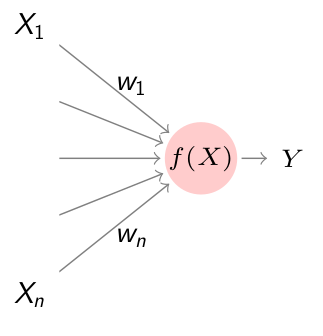
\includegraphics[width=0.28\textwidth]{fig/perceptron.png}
\caption{Perceptron.}
\label{fig:perceptron}
\end{figure}

\subsection{Multi-Layer Perceptron (MLP)}

Com novas camadas temos mais liberdade:
$$
Y =  \beta_0 + \sum_{k=1}^{K} \beta_k \, g\qty(w_{k0} + \sum_{j=1}^{p} w_{kj} X_k),
$$
onde $p$ é o número de variáveis na camada de input e $K$ o número de variáveis na camada oculta.
\begin{figure}[H]
\centering
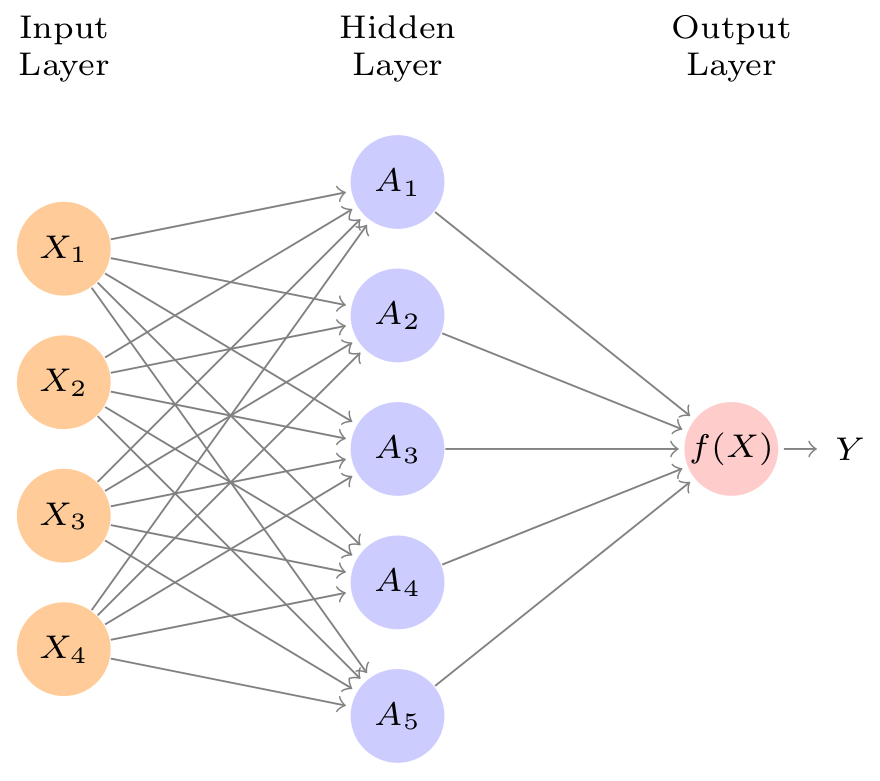
\includegraphics[width=0.4\textwidth]{fig/mlp.png}
\caption{Multi-Layer Perceptron (MLP).}
\label{fig:mlp}
\end{figure}

Com camadas oculta, a função de ativação $g(\cdot)$ deve ser não-linear, do contrário teremos uma estrutura linear. Geralmente escolhemos $g(z)$ assim (\texttt{ReLU} é mais comum nos dias de hoje):
\begin{figure}[H]
\centering
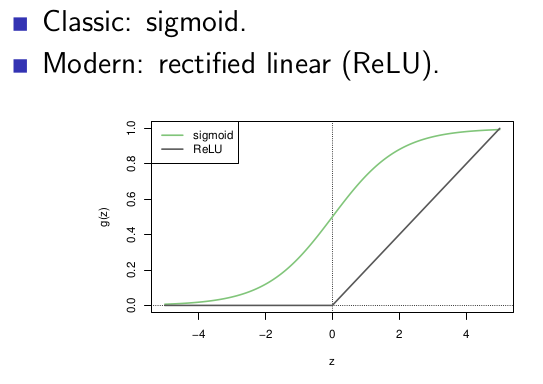
\includegraphics[width=0.4\textwidth]{fig/activation_function.png}
\caption{Função de ativação.}
\label{fig:units_activation_functions}
\end{figure}

Existe o chamado \textbf{Universal Approximation Result (1989)}: um Multi-Layer Perceptron (MLP) com uma única camada oculta consegue aproximar qualquer função contínua arbitrariamente bem.
\begin{figure}[H]
\centering
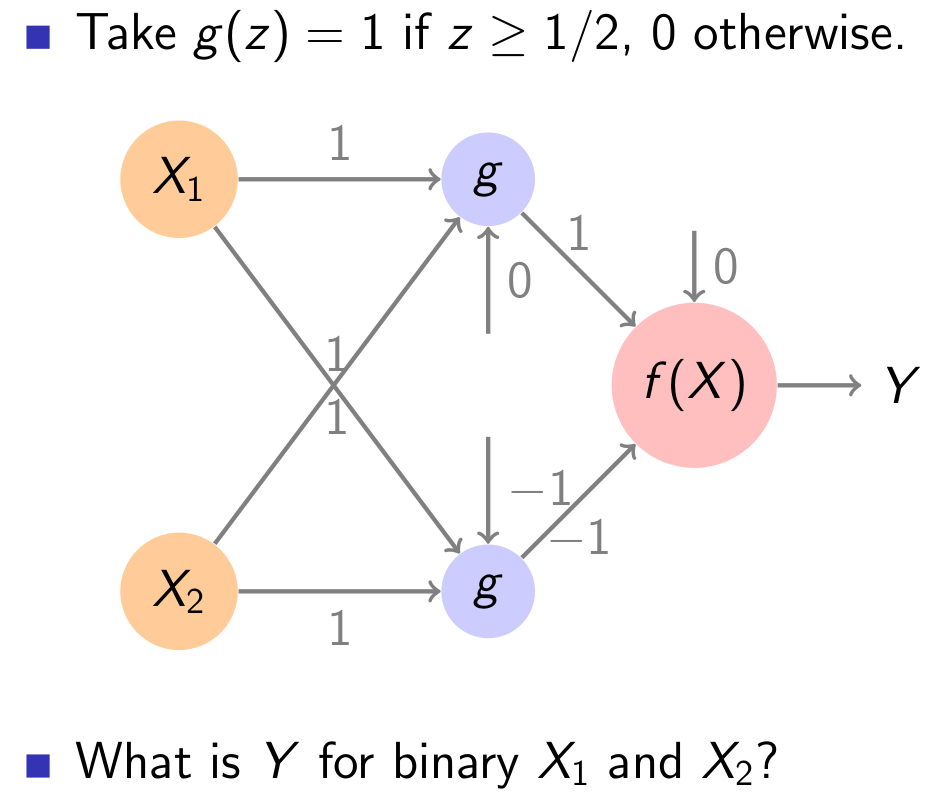
\includegraphics[width=0.4\textwidth]{fig/example_mlp.png}
\caption{Exemplo de Multi-Layer Perceptron (MLP).}
\label{fig:example_mlp}
\end{figure}

No exemplo acima, os pesos são:
$$
\begin{cases}
\; \beta_0 = 0, \beta_1 = 1, \beta_2 = -1; \\
\; w_{10} = 0 , w_{11} = 1, w_{12} = 1; \\
\; w_{20} = -1, w_{21} = 1, w_{22} = 1.
\end{cases}
$$
Isso nos dá que
$$
Y = g\qty(X_1 + X_2) - g\qty(X_1 + X_2 - 1),
$$
onde $g(z) = 1$ se $z \geq 1/2$ e $g(z) = 0$ caso contrário.

Com muitos outputs, a esquematização é desse jeito:
\begin{figure}[H]
\centering
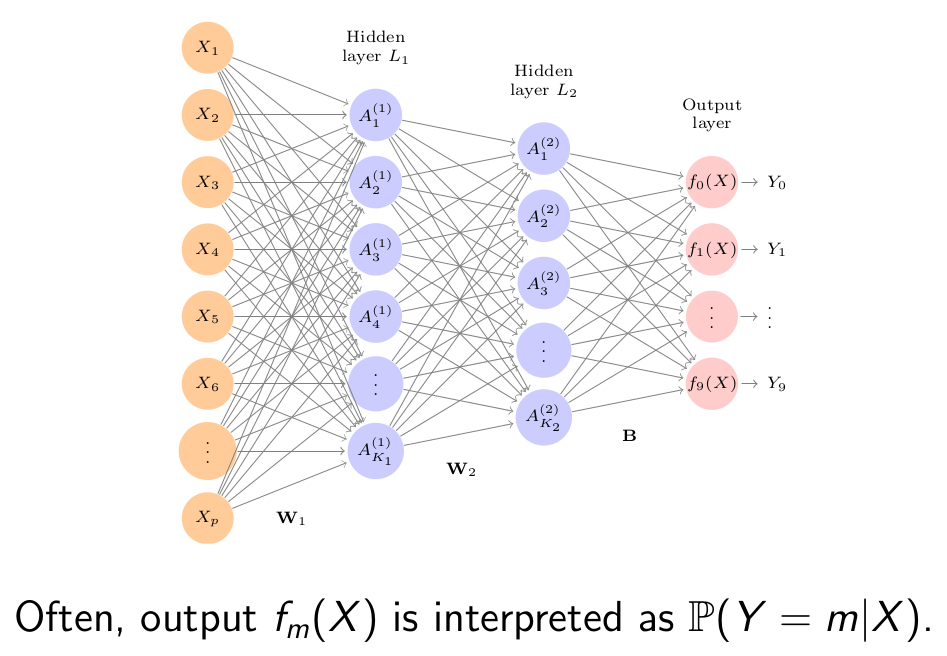
\includegraphics[width=0.6\textwidth]{fig/many_outputs.png}
\caption{Esquematização de muitos outputs.}
\label{fig:many_outputs}
\end{figure}

No caso de muitos outputs, por exemplo classificar uma imagem para saber qual dígito de 0-9 ela possui, é comum utilizarmos o \textit{one-hot coding}, usando assim 10 variáveis $Z_m$ com valores binários $m =$ 0 ou 1, ao invés de somente uma variável com 10 valores de 0-9.

Se todas os 10 outputs fossem separados e independentes, colocaríamos $f_m(X) = Z_m$ e seria isso mesmo, mas note que o \textit{one-hot coding} não é independente. Assim, interpretamos então $f_m(X) = \mathbb{P}(Y = m \mid X)$ e utilizamos a função especial \textit{softmax activation function}
$$
f_m(X) = \P(Y = m \mid X) = \frac{e^{Z_m}}{\sum_{\ell = 0}^9 e^{Z_\ell}}.
$$

Já que os outputs são qualitativos, para treinar esta rede tentamos estimar os coeficientes que minimizam a log-likelihood multinomial negativa
$$
- \sum_{i=1}^{n} \sum_{m=0}^{9} y_{im} \log(f_m(x_i)),
$$
também conhecida como \textit{cross-entropy}. Isso é uma generalização do critério de regressão logística para duas classes. Se os outputs fossem quantitativos, nós minimizaríamos o erro quadrático, como veremos na próxima seção.

\subsection{Treinando uma MLP}

Primeiro, escolher o número de camadas, número de variáveis em cada camada e as funções de ativação. Então, minimizamos o erro quadrático:
$$
R_\theta = \frac{1}{2} \sum_{j=1}^{N} (y_j - f_\theta(x_j))^2.
$$
O algoritmo que geralmente é usado em redes neurais para minimizar o erro quadrático é o \textit{gradiente descendente}. A cada iteração $t$, calculamos
$$
\grad{R_\theta^t} = \eval{\pdv{R_\theta}{\theta}}_{\theta^t}
$$
e tomamos $w^{t+1} = w^t - \rho \grad{R_\theta^t}$, onde $\rho$ é a \textit{taxa de aprendizado} (o número pequeno do gradiente descendente, nada demais).

Claramente, para calcularmos as derivadas de $R_\theta^t$, aplicamos a \textit{regra da cadeia} sem muito mistério.

Os algoritmos do estado da arte utilizam o \textit{gradiente descendente estocástico} para calcular as derivadas a partir de amostras dos dados selecionadas aleatoriamente.

Também é comum regularizar a minimização com ridge ou lasso:
$$
R(\theta; \lambda) = - \sum_{i=1}^{n} \sum_{m=0}^{9} y_{im} \log(f_m(x_i)) +
\lambda \sum_j \theta_j^2. \quad \text{(ridge)}
$$

\subsection{Dropout}

A ideia é do método de regularização \textit{dropout} é simplesmente remover aleatoriamente alguma das unidades (variáveis da camada de input) com probabilidade $p$ e reescalar todos as outras unidades por $\frac{1}{1-p}$ para compensar. É mais ou menos uma forma de fazer \textit{feature selection}.

\subsection{CNN e RNN}

Convolutional Neural Networks (CNN) são redes neurais (utilizadas para tratamento de imagens), só seus pesos $w_{kj}$ são mais estruturados. Interpretamos eles como sendo filtros convolucionais.
\begin{figure}[H]
\centering
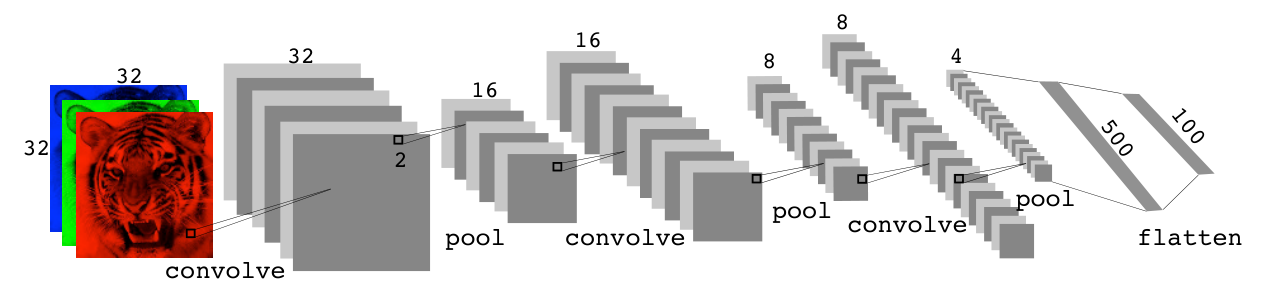
\includegraphics[width=0.6\textwidth]{fig/cnn_architecture.png}
\caption{Arquitetura de uma CNN.}
\label{fig:cnn_architecture}
\end{figure}

Recurrent Neural Networks (RNN) são redes neurais utilizadas para tratamento de dados sequenciais (por exemplo séries temporais).
\begin{figure}[H]
\centering
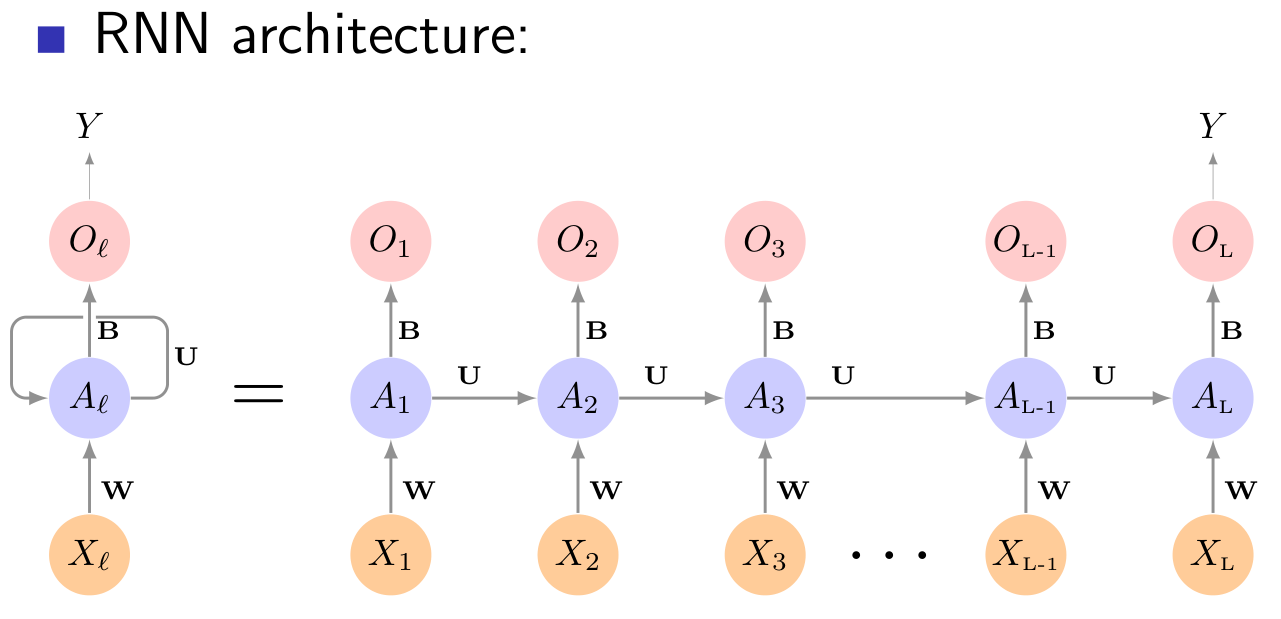
\includegraphics[width=0.5\textwidth]{fig/rnn_architecture.png}
\caption{Arquitetura de uma RNN.}
\label{fig:rnn_architecture}
\end{figure}

\subsection{Lembrete}

\begin{itemize}
\item Classificação: utilizamos \textit{softmax} e a \textit{cross-entropy}.
\item Regressão: utilizamos o erro quadrático.
\end{itemize}

\section{Árvores}

A ideia de métodos baseados em árvores é literalmente fazer um monte de \texttt{if} e \texttt{else} para ir classificando as coisas.
\begin{figure}[H]
\centering
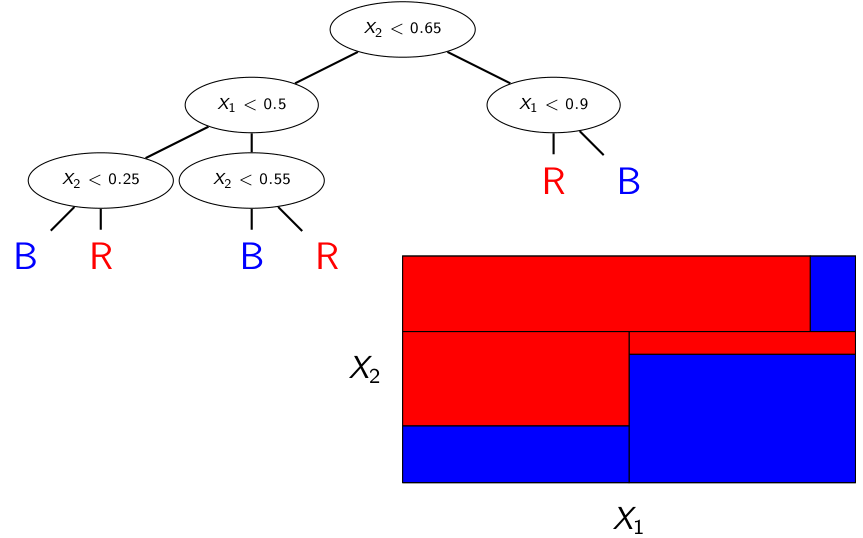
\includegraphics[width=0.8\textwidth]{fig/tree_method.png}
\caption{Método baseado em árvores.}
\label{fig:tree_method}
\end{figure}
É fácil de entender e desenhar, é flexível em capturar fronteiras e consegue lidar com features contínuas ou categóricas.

Para acharmos bons \textit{splits}, para \textit{árvores de regressão} existe a ideia básica (escolha o melhor split para cada passo de forma \textit{greedy}) e para \textit{árvores de classificação}, existe o algoritmo \texttt{C4.5}, que é baseado em entropia.

\subsection{Árvores de classificação}

Utilizamos o algoritmo \texttt{C4.5} para classificação.

A entropia de uma conjunto de observações $D$ é
$$
I(D) = - \sum_{k=1}^{K} p_k \log(p_k),
$$
onde $p_k = \abs{D_k} / \abs{D}$ e $D_k$ é o subconjunto de observações tal que $Y = k$.

O ganho de informação de uma partição de $D$ em datasets $D^1, \ldots, D^m$ é
$$
G(D^1, \ldots, D^m) = I(D) - \sum_{j=1}^{m} \frac{\abs{D^j}}{\abs{D}} \, I(D^j).
$$

Assim, o \textit{gain ratio} é $\frac{G(D^1, \ldots, D^m)}{I(D)}$.

\n

O algoritmo é
\begin{enumerate}
\item Input: dataset de treino.
\item Se o dataset está vazio, STOP. Se todos os labels no dataset forem idênticos, retornar uma \textit{leaf} com esse label.
\item Para cada split possível, computar a \textit{gain ratio} da partição resultante do dataset de treino.
\item \textit{Greedy step}: selecionar o split com maior \textit{gain ratio}.
\item O split corresponde a um nodo. Cada element da partição do dataset é uma aresta ao nodo possível. Passo recursivo: chamar o algoritmo para cada tal elemento.
\end{enumerate}

Suponha que tenhamos uma região contendo algumas observações coletadas no dataset $D$. O índice Gini dessa região é
$$
G = \sum_{k=1}^{K} \frac{\abs{D_k}}{\abs{D}} \qty(1 - \frac{\abs{D_k}}{\abs{D}}) = 1 - \sum_{k=1}^{K} \qty(\frac{\abs{D_k}}{\abs{D}})^2.
$$
Ele não é nada mais do que expandir o log em primeira ordem em Taylor (entropia linear) e é uma medida de pureza (assim como na Mecânica Quântica, para a matriz densidade).

Podemos avaliar um split com a entropia ou com Gini index (que é uma aproximação da entropia).

\subsection{Árvores de regresão}

No caso de $Y$ ser uma variável contínua, a ideia é a mesma: fazer splits de forma \textit{greedy}, só que dessa vez minimizamos o RSS
$$
\sum_{j=1}^{J} \sum_{i \in R_j} (y_i - \hat{y}_{R_j})^2.
$$

Em cada passo, para cada $j$ e $s$ nós definimos os pares
$$
R_1(j, s) = \qty{X \mid X_j < s} \e R_2(j, s) = \qty{X \mid X_j \geq s},
$$
e procuramos os valores de $j$ e $s$ que minimizam a expressão
$$
\sum_{i : \, x_i \in R_1(j, s)} (y_i - \hat{y}_{R_1})^2 +
\sum_{i : \, x_i \in R_2(j, s)} (y_i - \hat{y}_{R_2})^2.
$$
No próximo passo, ao invés de splitar o espaço inteiro, nós splitamos uma das duas regiões identificadas previamente. O processo continua até um critério de parada ser satisfeito.

O processo descrito acima pode ter bons resultados no dataset de treino, mas é bem provável que aconteça um overfitting. Isso é porque a árvore resultante pode acabar sendo muito complexa.

Uma boa estratégia é montar uma árvore grande $T_0$ e depois cortá-la para obter uma sub-árvore menor.

Podemos selecionar um pequeno subconjunto de sub-árvores através do \textit{cost complexity pruning}. Nós consideramos uma sequência de árvores indexadas por um parâmetro $\alpha \geq 0$. Para cada valor de $\alpha$ corresponde uma sub-árvore $T \subset T_0$ tal que
$$
\sum_{m=1}^{\abs{T}} \sum_{i: \; x_i \in R_m} (y_i - \hat{y}_{R_m})^2
+ \alpha \abs{T}
$$
é o mínimo possível. Aqui, $\abs{T}$ indica o número de \textit{leaves} da árvore $T$. O parâmetro $\alpha$ controla o trade-off entre a complexidade da árvore e o seu fit ao dataset de treino. A ideia então é selecionar vários valores de $\alpha$ e aplicar validação cruzada para tuná-lo para o melhor possível que minimizar o erro médio.

\subsection{Vantagens e desvantagens}

\textbf{Vantagens:}
\begin{itemize}
\item Árvores são fáceis de entender.
\item Podem ser traduzidas em ``regras''.
\item São mais flexíveis que regressão logística (basicamente linear).
\item Conseguem lidar com variáveis contínuas ou categóricas.
\end{itemize}

\textbf{Desvantagens:}
\begin{itemize}
\item Não têm muita acurácia.
\item Não são robustas; muito sensíveis ao dataset de treino (variância é grande).
\end{itemize}

\subsection{Bagging trees}

Uma única árvore é boazinha. Mas por que não aprender um conjunto de árvores e fazer a média dos resultados? Essa ideia leva a \textit{bagging trees} e \textit{random forests}.

Bagging é o seguinte. Pegamos o dataset de treino e produzimos $B$ amostras dele próprio através de \textit{bootstrap}. Então tomamos a média para regressão e a maioria por votos para classificação. Isso é \textit{bagging}, e funciona para qualquer tipo de classificador. Geralmente é aplicado para \textit{weak classifiers}, que sozinhos não são muito bons mas com \textit{bagging} o resultado é melhorado. Esse é o caso para árvores de classificação ou regressão.

Para estimar o erro utilizando \textit{bagging}, não é necessário fazer validação cruzada. Basta que, para cada observação, nós produzimos a média de todas as árvores que foram aprendidas sem essa observação no conjunto de treino. Assim computamos o erro médio para essa observação. Isso é uma boa estimativa do erro, e quando $B \to \infty$ este erro tende ao erro do leave-one-out cross validation.

\subsection{Random forests}

O método de \textit{random forest} é dentro do contexto de \textit{bagging}. Só que, todavez ao fazer um split, nos restringimos a um subconjunto de $m$ features (das $p$ features/predictors $X_1, \ldots, X_p$) escolhido aleatoriamente para realizar o splitting. Normalmente toma-se $m \approx \sqrt{p}$.

Pela influência aleatória dos splis, as árvores tornam-se mais descorrelacionadas com as outras. Pela diminuição de correlação, a variância é reduzida.

Note que se tomássemos $m = p$ isso se reduziria ao caso normal de \textit{bagging}, já que qualquer split possível seria considerado.

Geralmente \textit{random forests} apresentam uma pequena melhoria com relação ao \textit{bagging} normal.

\subsection{Boosting}

\textit{Boosting} é um método geral para melhorar os resultados de um conjunto de \textit{weak classifiers} $g_k(X)$ (eles são fracos no sentido de que podem ser um pouco melhor do que chutes aleatórios, mas podem em tese ter boa acurácia se disponível).

A ideia de \textit{boosting} é combinar eles de maneira a produzir um classificador mais foda. Enquanto $g_1$ é aprendido no training dataset original, cada $g_k$ é aprendido numa versão ponderada do dataset original. Em outras palavras, sendo a variável de classe $Y \in \qty{-1,1}$, o \textit{boosted classifier} é
$$
g(x) = \text{sign}\qty(\sum_{k=1}^{M} \alpha_k g_k(x)),
$$
para alguns $\alpha_k$.

Ideia simples:
\begin{itemize}
\item Aprender $g_1$.
\item Aprender $g_2$, enfatizando que deve fazer a coisa certa quando $g_1$ cometer um erro.
\item Aprender $g_3$, enfatizando que deve fazer a coisa certa quando $g_1$ ou $g_2$ cometerem um erro. And so on...
\end{itemize}

O algoritmo mais famoso é o \texttt{AdaBoost}:
\begin{enumerate}
\item Inicializar $w_j = 1/N$, para $j \in \qty{1,\ldots,N}$.
\item Para $k$ de $1$ a $M$:
\begin{enumerate}
\item Aprender $g_k(X)$ no training dataset usando os pesos $w_j$.
\item Calcular
$$
\beta_k = \frac{\sum_{j=1}^{N} w_j \, I_{y_j \neq g_k(x^j)}}{\sum_{j=1}^{N} w_j}.
$$
\item Calcular $\alpha_k = \ln(\frac{1-\beta_k}{\beta_k})$.
\item Multiplicar cada peso $w_j$ por $\exp(\alpha_k I_{y_j \neq g_k(x^j)})$.
\end{enumerate}
\item Output $g(x) = \text{sign}\qty{\sum_{k=1}^{M} \alpha_k g_k(x)}$.
\end{enumerate}

Um esquema popular é utilizar \textit{boosting} com \textit{stumps} (troncos: árvores com um único split). Boosted classifiers com um grande número de stumps funciona muito bem.

\end{document}
